\chapter{Monopole design}

A monopole antenna is one of the most simple antenna structures, as it is just a wire, where the signal generator is connected at one end, place atop of a ground plane. The theoretic radiation pattern can be seen on \autoref{fig:disMono}. As the ground plane is not perfect in reality, the shape might distort by either changing the tilt or going towards a more doughnut shape.

\begin{figure}[H]
\centering
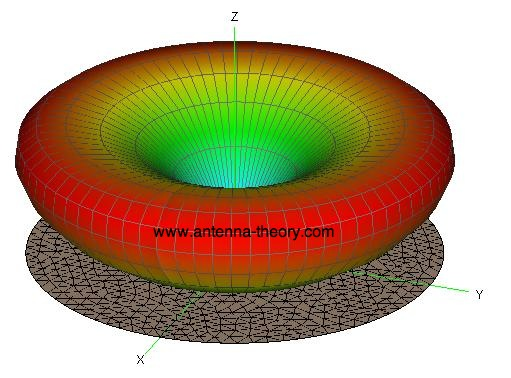
\includegraphics[width=0.5\textwidth]{figure/disturbedMonopole.jpg}
\caption{Radiation pattern of a quarter length monopole antenna, with a ground plane with a diameter on 3 wavelength.}
\label{fig:disMono}
\end{figure}

The frequency of the monopole antenna is determined by the length of the antenna, like the dipole antenna. The antenna needs a length equal to a forth of the wavelength of the wanted frequency, which is equal to half the size of a dipole antenna, with same frequency. With this length, it will have a input impedances on $(36.5 + 21.25j) \ohm$.

\begin{equation}\label{eq:lengthMono}
L = \frac{\lambda}{4}
\end{equation}
\begin{where}
\va{$L$}{is the length of the antenna}{m}
\va{$\lambda$}{is the wavelength of the wanted frequency}{m}
\end{where}

\section{Dimensions of Monopole Antennas}

The monopole antennas have been designed with the dimensions

\begin{table}[H]
\centering
\begin{tabular}{l|lll}
                				& \textbf{858MHz} 	& \textbf{2.58GHz} 	& \textbf{Unit} \\\hline
\textbf{Height}  				& 87           		& 29            	& mm            \\
\textbf{Width of ground plane} 	& 130            	& 60            	& mm 
\end{tabular}
\caption{Calculated parameters}
\label{tab:parameters}
\end{table}


\begin{figure}[H]
\captionsetup{belowskip=0em}
\begin{subfigure}[b]{0.48\textwidth}
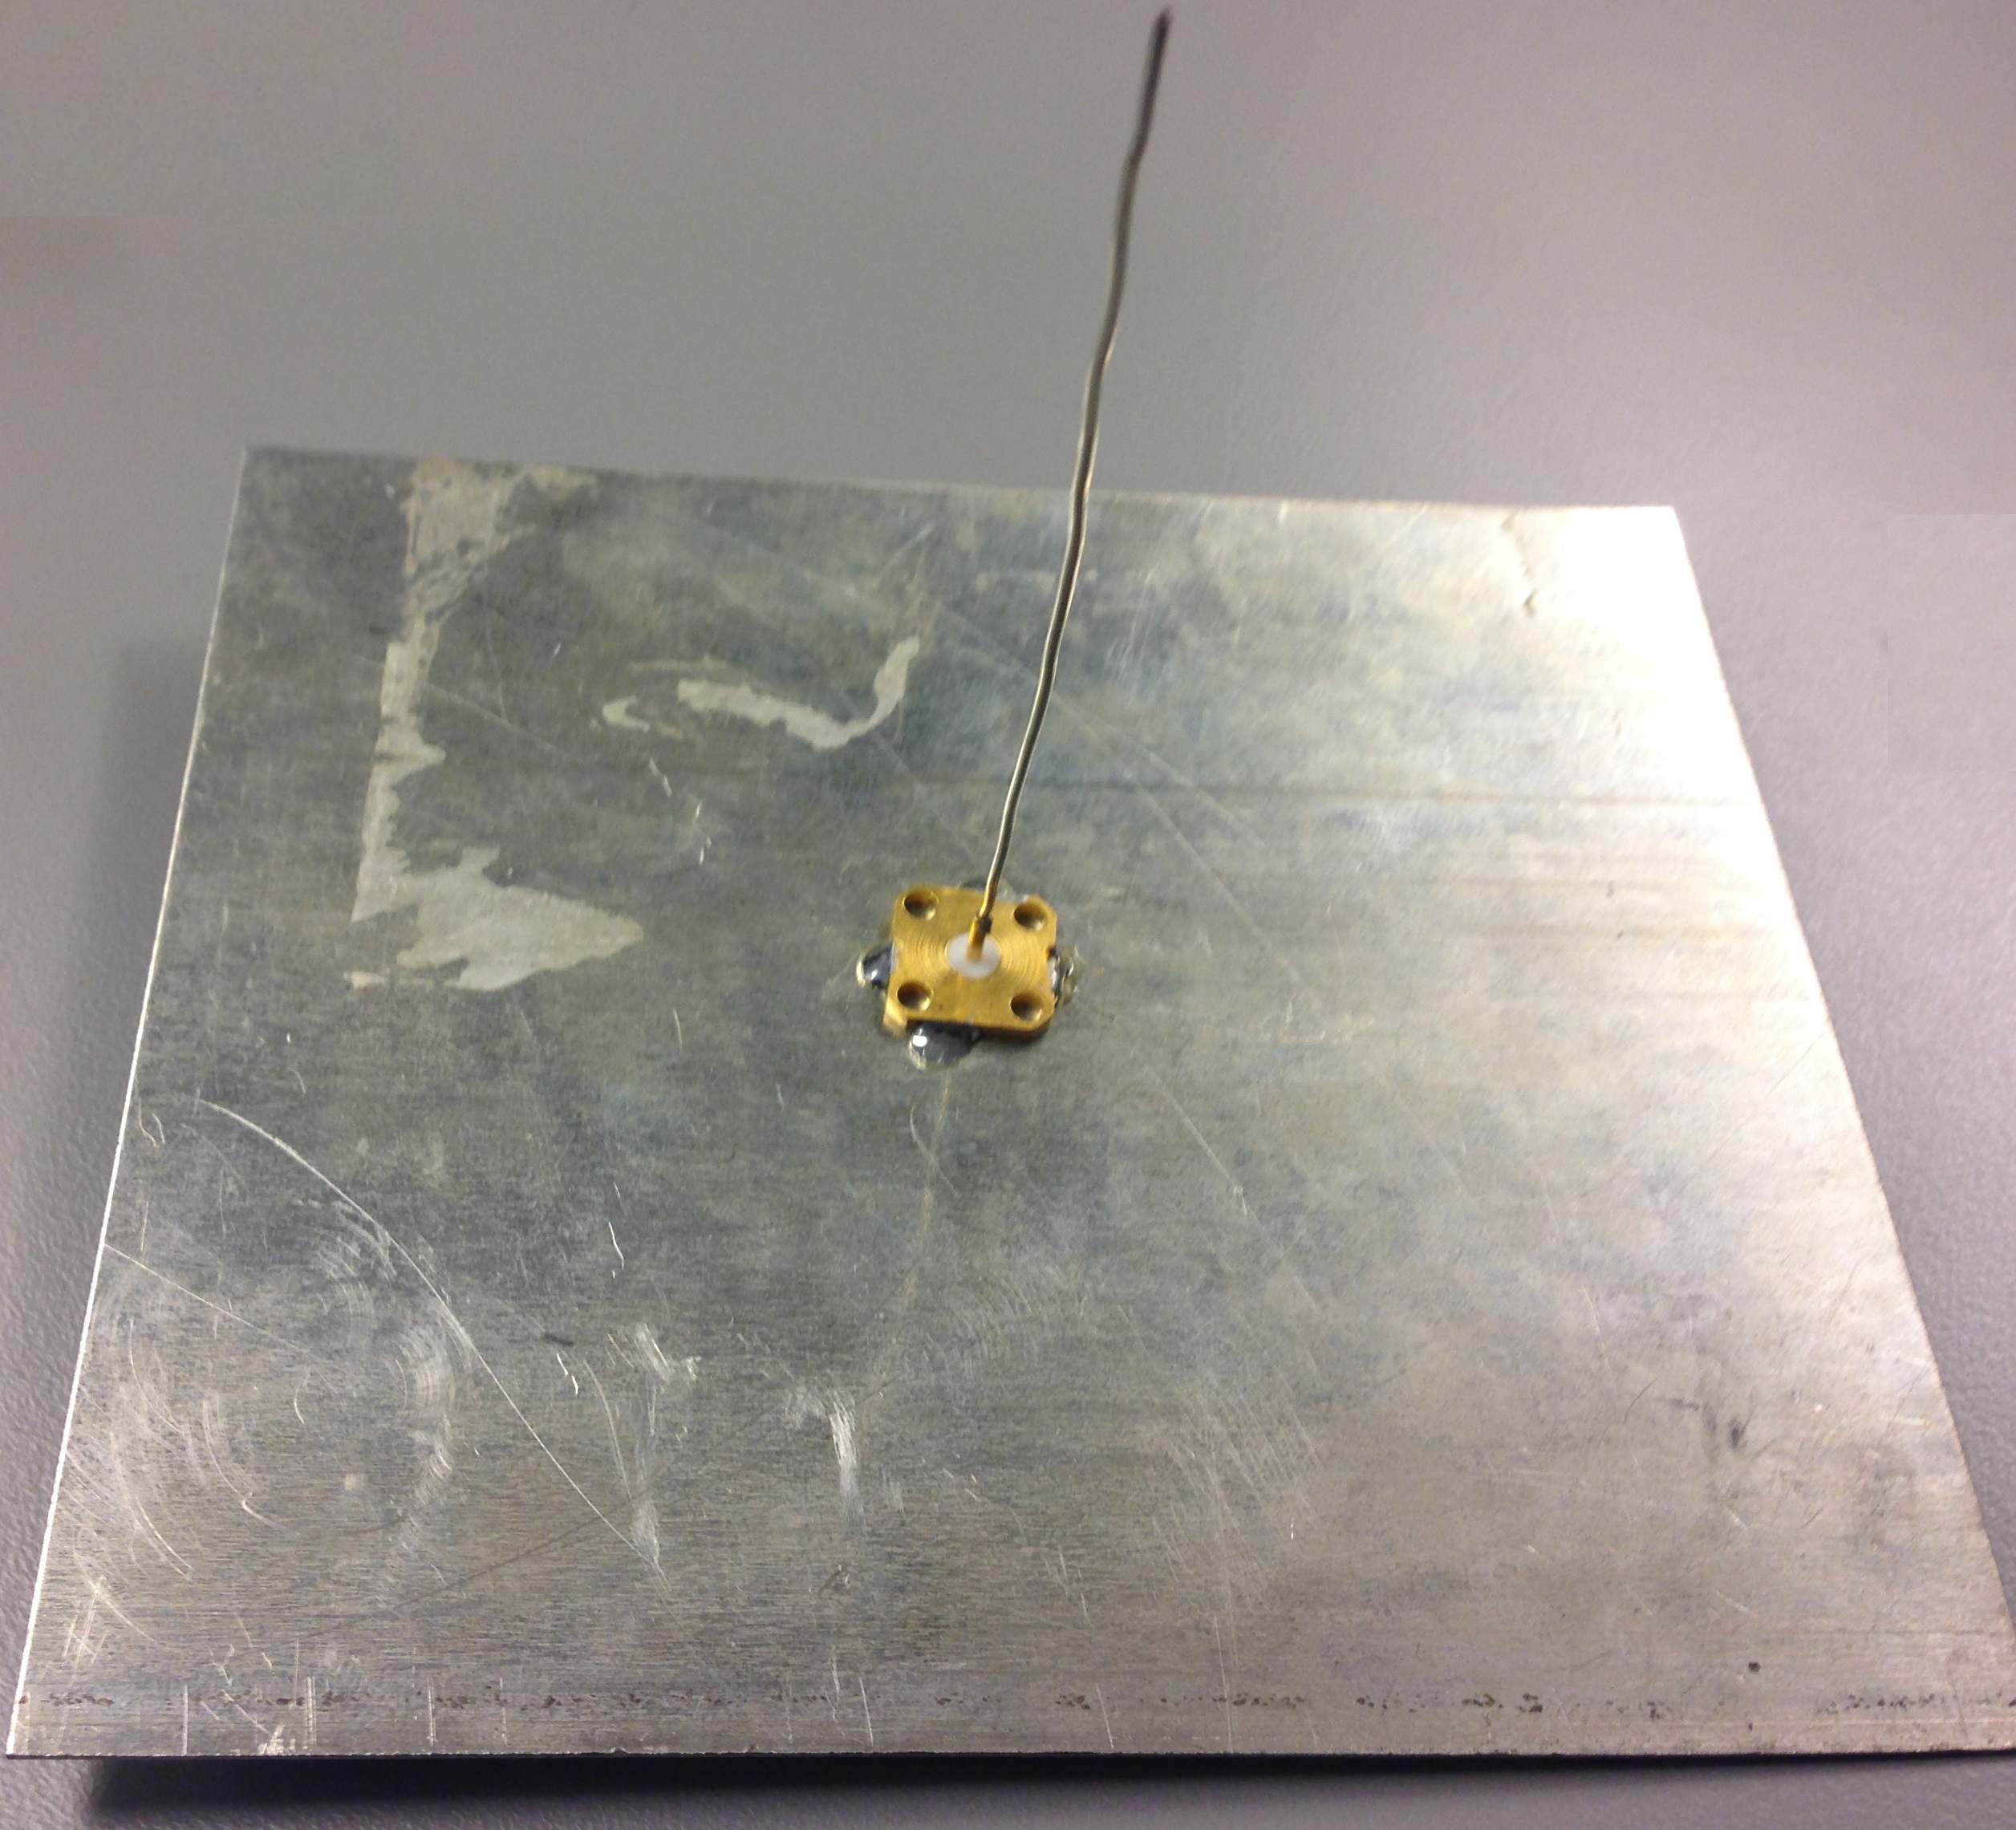
\includegraphics[width=\textwidth]{figure/IMG_0918.jpg}
\caption{Designed monopole for 858 MHz}
\label{fig:868Patch}
\end{subfigure}
\begin{subfigure}[b]{0.48\textwidth}
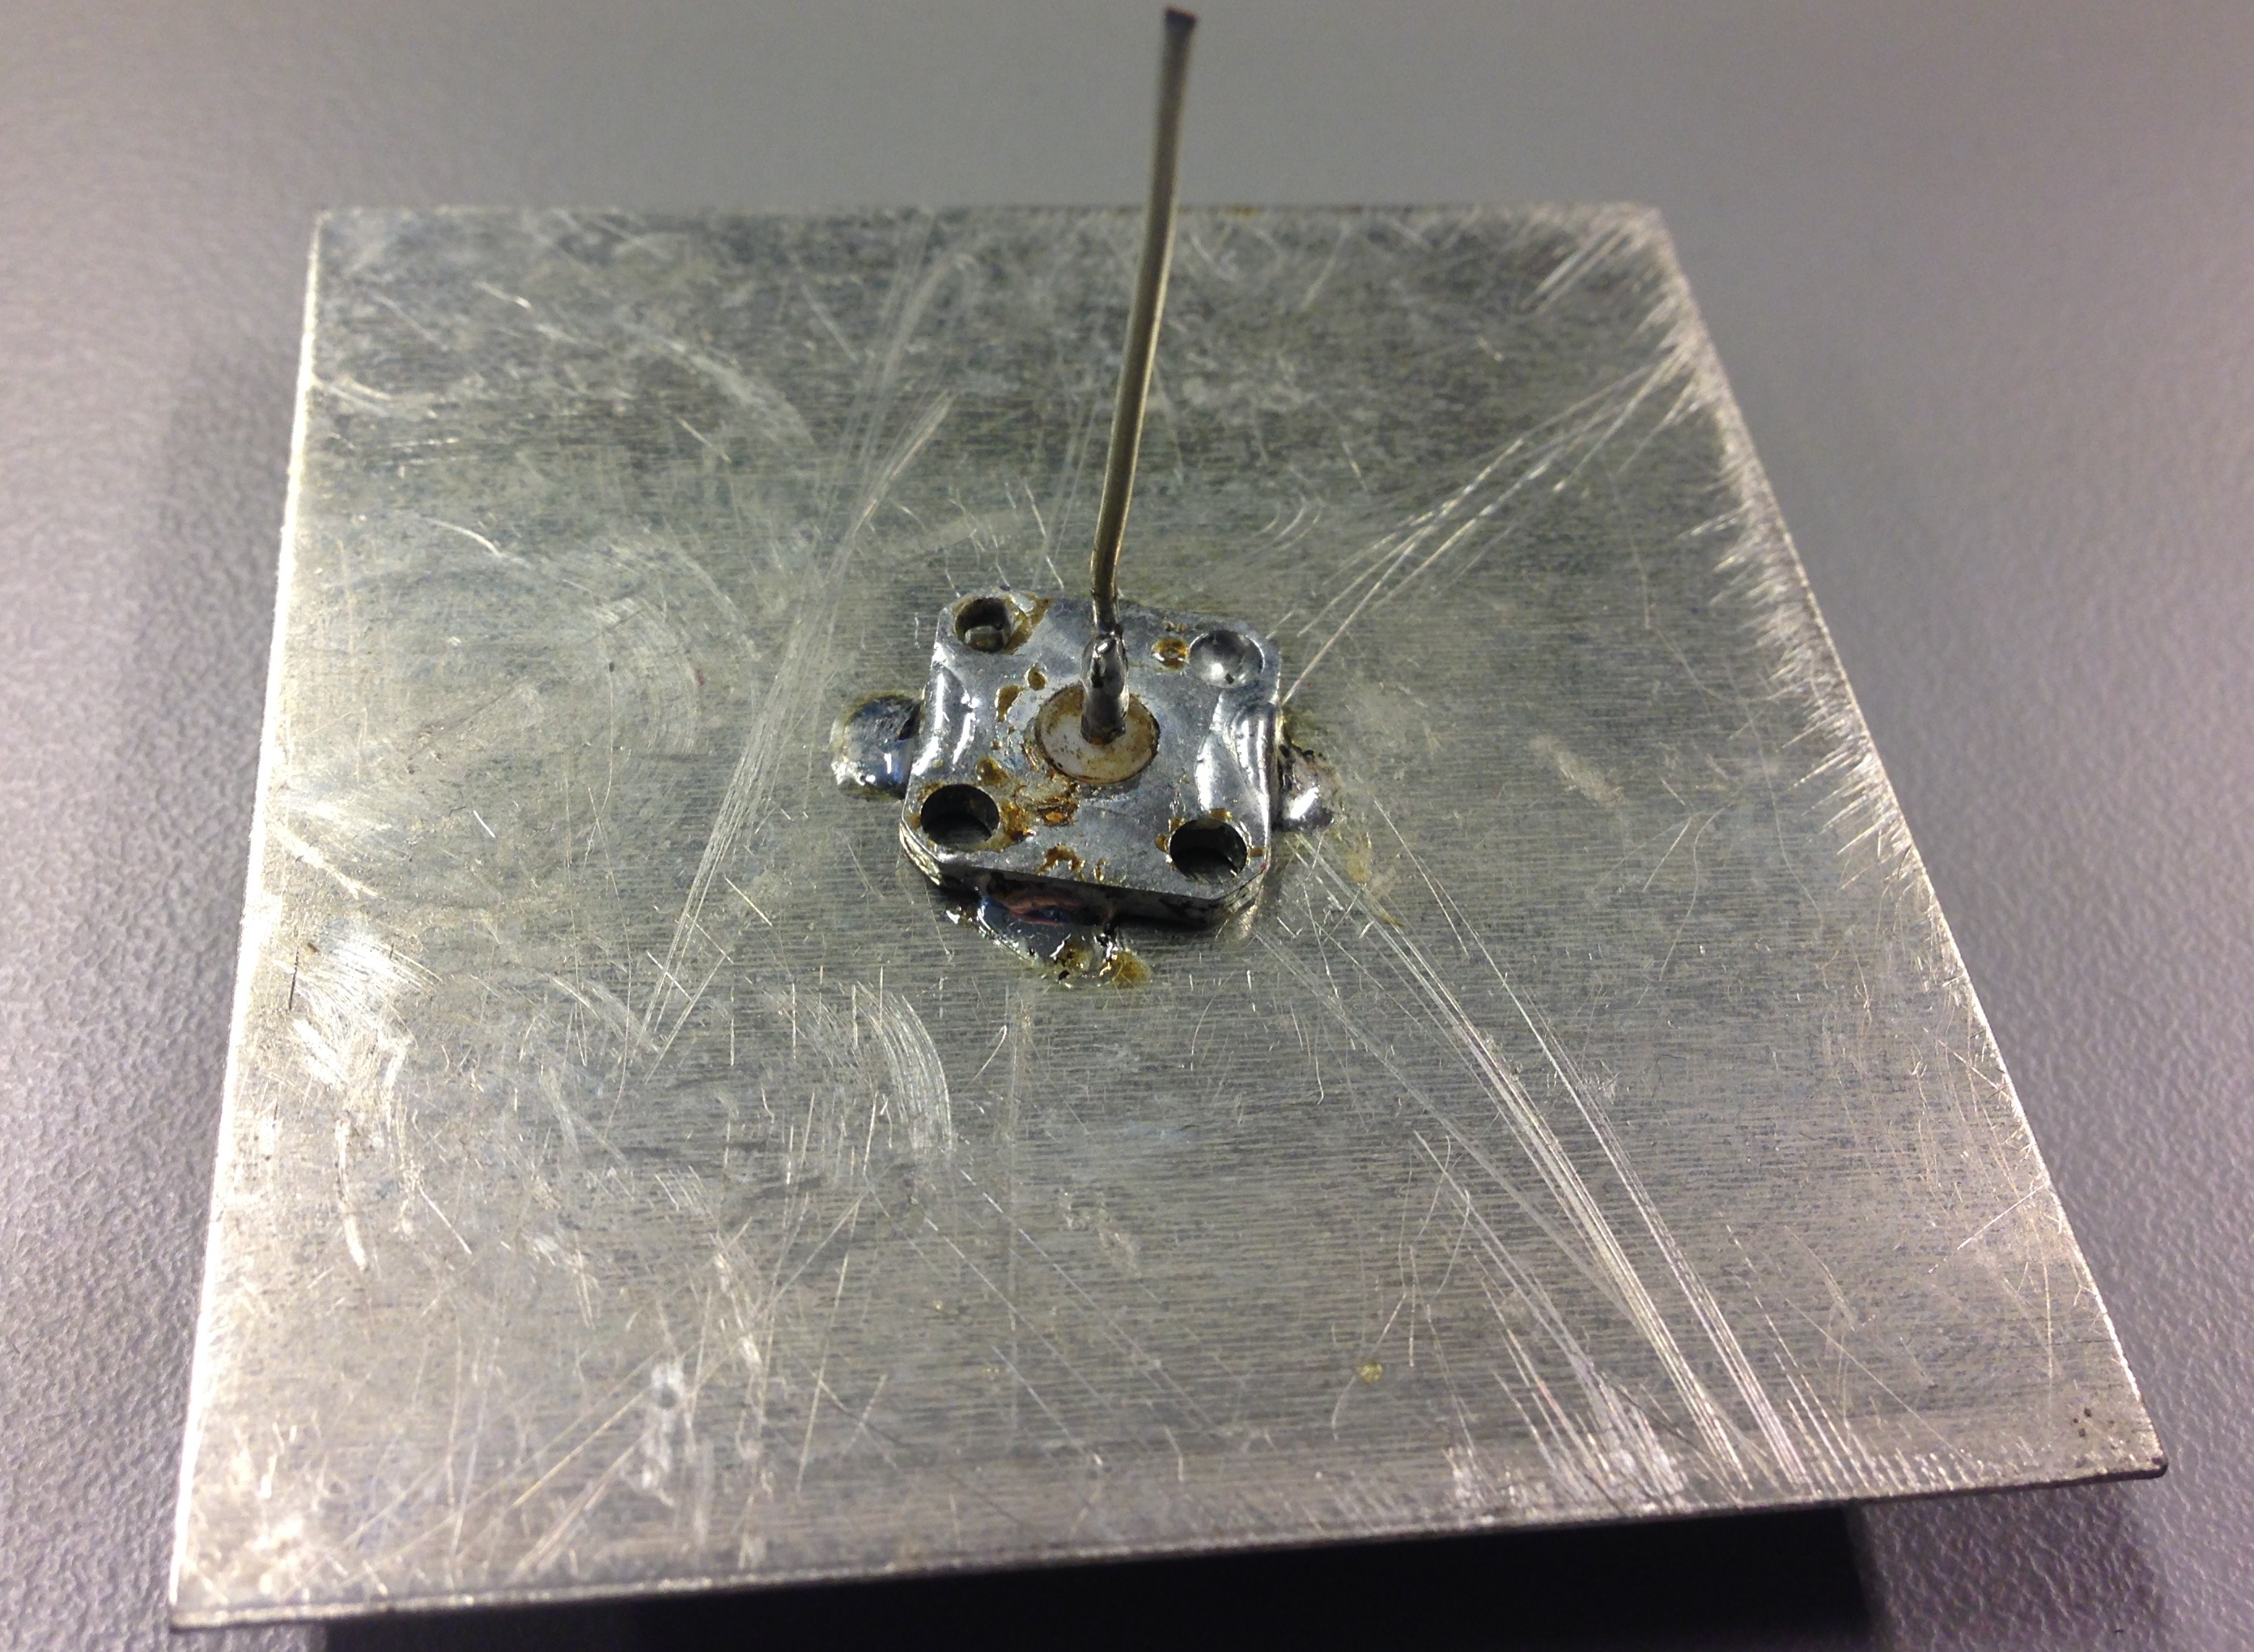
\includegraphics[width=\textwidth]{figure/IMG_0919.jpg}
\caption{Designed monopole for 2.58 GHz}
\label{fig:2.4Patch}
\end{subfigure}
\captionsetup{belowskip=-1.5em}
\caption{The manufactored monopole antennas}
\end{figure}